\documentclass{article}
\usepackage{tikz-cd}
\usepackage{hyperref}
\usepackage{amsmath}
\usepackage{amssymb}
\usepackage{booktabs}
\usepackage{siunitx}

% For BibTex
\usepackage[round]{natbib}
\bibliographystyle{apalike}
\hypersetup{citecolor = blue}

% To modify margins
\usepackage[margin = 1in]{geometry}
\setlength{\parindent}{0pt}
\setlength{\parskip}{1em}

% Title specific margins
\usepackage{titling}
\setlength{\droptitle}{-6em}

% Add figures with borders
\usepackage{graphicx}
\usepackage{tcolorbox}
\usepackage{caption}
\usepackage[labelfont = bf]{caption}

\title{Congestive Heart Failure Classification \vspace{-2ex}}
\author{Weslee Nguyen and Sedona O'Hearn | DATA474 | Professor Qian}
\date{}

%%%%%%%%%%%%%%%%%%%%%%%%%%%%%%%%%%%%%%%%%%%%%%%%%%%%%%%%%%%%%%%%%%%%%%%%%
%%%%%%%%%%%%%%%%%%%%%%%%%%%%%%%%%%%%%%%%%%%%%%%%%%%%%%%%%%%%%%%%%%%%%%%%%
%%%%%%%%%%%%%%%%%%%%%%%%%%%%%%%%%%%%%%%%%%%%%%%%%%%%%%%%%%%%%%%%%%%%%%%%%

\begin{document}

\maketitle
\vspace{-20mm}
\section*{Introduction}
\vspace{-6mm}
The Biopsychosocial Model (BPSM) posits that psychological, biological, and social factors all impact one another to give rise to disease \citep{BPSM2023}. While touted as a key model where providers consider a diverse array of factors that cause and impact disease, the theory is often criticized as too vacuous. For example, a given disease could have primarily biological causes, have little psychosocial interactions, or clinicians may only need to evaluate social, but not biological factors. We focus on Congestive Heart Failure (CHF), a syndrome already known to have biological (adult males, hypertension, coronary artery disease), psychological (anxiety, depression, diet), and social (family history, socioeconomic status, healthcare access) factors, to name a few \citep{CHFPathophysiology2021, CHF-BPSM2025}. Thus, exploring the magnitude factors can predict whether someone has or had CHF and their interactive effects can give insight into the utility of BPSM.

The National Health and Nutrition Examination Survey (NHANES) is an American nationwide survey that provides comprehensive subjective and objective scores relating to demographics, the environment, and physical and mental health \citep{CHF-NHANESA2024}. Over ten thousand participants are involved in the program every two years, though collection stopped during COVID. As of writing, the most recent two year cycle's data and documentation for August 2021-August 2023 has been fully processed and released to the public, of which participants were asked ``Has a doctor or other health professionals ever told that you had congestive heart failure?''

As a result, one can consider the swaths of biological and environmental factors in creating a classification model of whether or not someone has or had CHF. While this model cannot be considered a diagnostic tool to aid clinicians, this can be used to evaluate the predictiveness of various factors, particularly in tandem, that can lead to CHF. Thus, this report can be viewed as a specific case study in evaluating the BPSM.

\vspace{-6mm}
\section*{Methods}
\vspace{-6mm}

Due to the onslaught of factors, the involving datasets have been obtained for this project: demographics (DEMO$\_$L), diet (DR2TOT$\_$L), blood pressure (BPXO$\_$L), body measures (BMX$\_$L), mental health (DPQ$\_$L), medical conditions (MCQ$\_$L), physical activity (PAQ$\_$L), diabetes (DIQ$\_$L), cigarette use (SMQ$\_$L), standard biochemistry profile (BIOPRO$\_$L), complete blood count (CBC$\_$L), albumin and creatinine (ALB$\_$CR$\_$L), and environmental chemical exposure (PBCD$\_$L) (being lead, cadmium, total mercury, selenium, and manganese). Each dataset was downloaded from the CDC website for NHANES and converted from xpt to csv. The following preprocessing steps were taken:

\begin{enumerate}
	\item Merge all datasets via SEQN, which is the unique identification number per participant.
	\item Retain only participants 18 years or older.
	\item Only retain participants who explicitly answered Y/N to having CHF (nearly 4,000 didn't respond).
	\item Drop empty predictors (has $> 30\%$ lack responses).
	\item To impute (MICE), remove highly multicollinear columns. Groups where each variable had $>95\%$ correlation was reduced down to one variable, which was chosen randomly.
	\item Perform multiple imputation with chained equations (MICE) with predictive mean matching (PMM).
\end{enumerate}

Due to step (\textbf{4}) and (\textbf{5}), the dataset was reduced (p = 204, n = 6055). Most predictors removed had child-specific measurements (e.g. head and arm circumference, child dietary recalls), follow-up variables (e.g. had and still have thyroid problems), and converting measurements (e.g. eosinophilic percent to count). 

%%%%%%%%%%%%%%%%%%%%%%%%%%%%%%%%%%%%%%%%%%%%%%%%%%%%%%%%%%%%%%%%%%%%%%%%%
%%%%%%%%%%%%%%%%%%%%%%%%%%%%%%%%%%%%%%%%%%%%%%%%%%%%%%%%%%%%%%%%%%%%%%%%%
%%%%%%%%%%%%%%%%%%%%%%%%%%%%%%%%%%%%%%%%%%%%%%%%%%%%%%%%%%%%%%%%%%%%%%%%%

For exploratory data analysis (EDA), a correlation matrix was performed with all the remaining predictors with CHF. The top ten predictors wtih the highest correlation magnitudes with CHF was taken, where a histogram was taken and the magnitudes of predictor values of those with and without CHF was taken (Fig. 1, Table 1). A paired t-test was taken (Table 1).

\vspace{-6mm}
\section*{Results}
\vspace{-6mm}

We see from EDA that the top ten predictors correlating with CHF probability is having prior medical conditions already known to be associated with CHF, an BMI-associated index, and various laboratory measures known to be associated with CHF. They are all positively associated with increased risk for CHF save for Blood Urea Nitrogen (BUN) which is negatively associated (Fig. 1), where these associations are all statistically significant, though with over 6,000 participants in the dataset, the t-statistics would be inflated (Table 1). Thus, effect sizes were calculated with notable increases, where having had (or still having) CHF is associated with an over 15 times increase having had experienced a heart attack. Yet there's a lack temporally sequential information that can determine if these measures then change CHF likelihood or vice versa, thus no inference on casuality can be mode. However, these associations mean that we expect prior medical history and lab work are included in the predictive CHF model in spite of aggressive methods prioritizing parsimony.

\begin{center}
\begin{tcolorbox}[colframe=black, colback=white, boxrule=0.5pt, arc=6pt, width=\textwidth]
	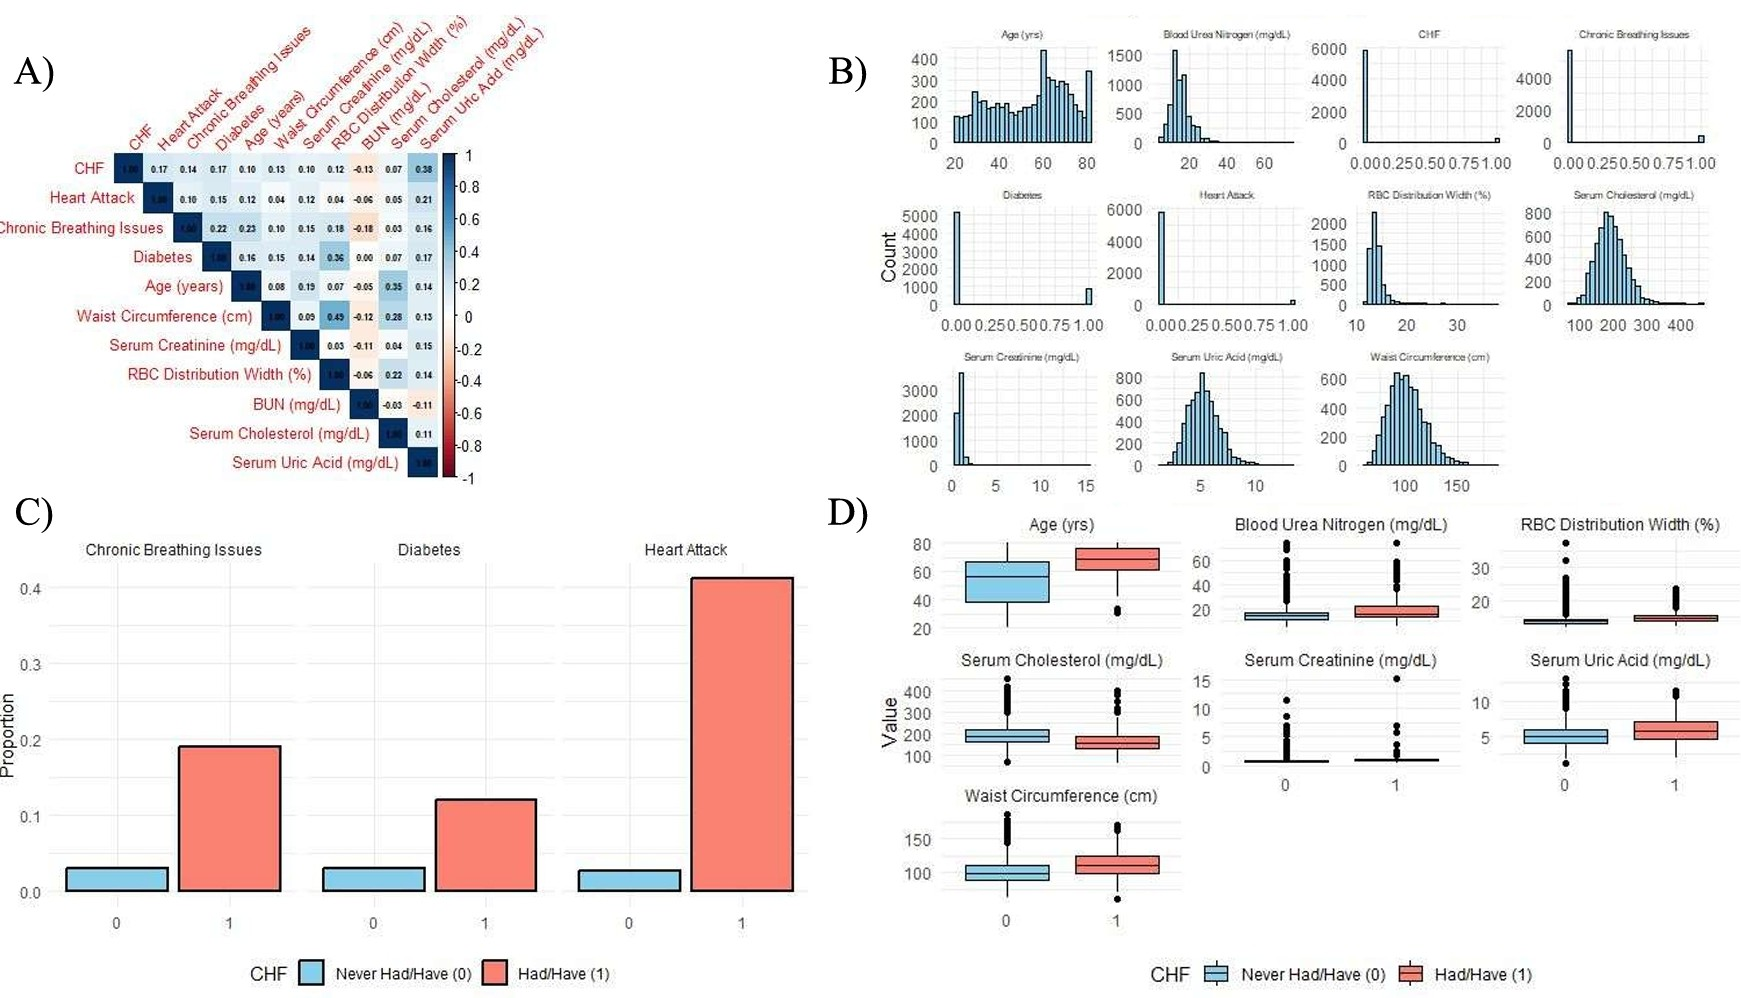
\includegraphics[width=\textwidth]{Fig_1.jpeg}
	\centering
	\captionof{figure}{Top ten predictors correlated with a participant who had / has CHF. (\textbf{A}) The upper triangular correlation matrix is shown of the top ten variables with the highest correlation magnitudes with CHF. (\textbf{B}) The histograms of each ten variables plus CHF are shown. (\textbf{C}) The proportion of participants reporting a chronic breathing disease (COPD, emphysema, and / or chronic bronchitis), Type I/II diabetes, or prior heart attack, and (\textbf{D}) the distribution of participants reporting age, waist circumference, and various lab measurements, was compared between those with and without CHF.}
\end{tcolorbox}
\end{center}
\vspace{-4mm}

\begin{center}
\begin{tcolorbox}[colframe=black, colback=white, boxrule=0.5pt, arc=6pt, width=\textwidth]
	\centering

\begin{tabular}{lllS} \toprule
     & {$\overline{CHF}_0$} & {$\overline{CHF}_1$} & {$\overline{CHF}_1 / \overline{CHF}_0$}  \\ \midrule
    \text{Heart Attack}  & 0.026 $\pm$ 0.002 & 0.407 $\pm$ 0.031 & 15.728  \\
    \text{Chronic Breathing Issues}  & 0.062 $\pm$ 0.003 & 0.329 $\pm$ 0.029 & 5.290  \\ \midrule
    \text{Diabetes}  & 0.131 $\pm$ 0.226  & 0.403 $\pm$ 0.031 & 3.079  \\ 
    \text{Age (yrs)}  & 53.210 $\pm$ 0.226  & 67.740 $\pm$ 0.612 & 1.273  \\ \midrule
    \text{Waist Circumference (cm)}  & 100.757  $\pm$ 0.222 & 112.545 $\pm$ 1.185 & 1.117 \\
    \text{Serum Creatinine (mg/dL)}  & 0.888 $\pm$ 0.005 & 1.150 $\pm$ 0.067 & 1.295  \\ \midrule
    \text{RBC Distribution Width (\%)}  & 13.825 $\pm$ 0.017 & 14.857 $\pm$ 0.115 & 1.075 \\ 
    \text{Blood Urea Nitrogen (mg/dL)}  & 15.001 $\pm$ 0.074 & 19.093 $\pm$ 0.590 & 1.273 \\ \midrule
    \text{Serum Cholesterol (mg/dL)}  & 191.004 $\pm$ 0.563 & 166.547 $\pm$ 2.978 & 0.872 \\ 
    \text{Serum Uric Acid (mg/dL)} & 5.117 $\pm$ 0.0182 & 5.868 $\pm$ 0.106 & 1.147  \\  \bottomrule
\end{tabular}
\par\vspace{1em}\par
\begin{tabular}{lSSll} \toprule
     & {$\overline{CHF}_1 - \overline{CHF}_0$} & {Statistic} & {p-value} & {CI} \\ \midrule
    \text{Heart Attack} & 0.381 & 12.408 & $<<<$0.01 & [0.321, 0.442] \\
    \text{Chronic Breathing Issues} & 0.267 & 9.060 & $<<<$0.01 & [0.209, 0.325]  \\ \midrule
    \text{Diabetes} & 0.272 & 8.803 & $<<<$0.01 & [0.211, 0.333] \\ 
    \text{Age (yrs)} & 14.531 & 22.278  & $<<<$0.01 & [13.248, 15.813]     \\ \midrule
    \text{Waist Circumference (cm)} & 11.788 & 9.779 & $<<<$0.01 & [9.415, 14.162] \\
    \text{Serum Creatinine (mg/dL)} & 0.262 & 3.915 & 0.0001 & [0.130, 0.394]  \\ \midrule
    \text{RBC Distribution Width (\%)} & 1.033  & 8.855 & $<<<$0.01 & [0.803, 1.262]  \\ 
    \text{Blood Urea Nitrogen (mg/dL)} & 4.092 & 6.877 & $<<<$0.01 & [2.920, 5.264]  \\ \midrule
    \text{Serum Cholesterol (mg/dL)} & -24.457 & -8.069 & $<<<$0.01 & [-30.424, -18.490]  \\ 
    \text{Serum Uric Acid (mg/dL)} & 0.751 & 6.969 & $<<<$0.01 & [0.539, 0.963]  \\  \bottomrule
\end{tabular}

\captionof{table}{Comparison of top ten CHF-correlated variables: mean / proportion ± SE by CHF status, ratios, differences, test statistics, p-values, and 95\% confidence intervals. $<<<$0.01 means $<1*10^{-10}$}
\end{tcolorbox}
\end{center}

fdsa

\vspace{-6mm}
\section*{Discussion}
\vspace{-6mm}

fdsa

\vspace{-6mm}
\section*{Conclusion}
\vspace{-6mm}

fdsa

\bibliography{NHANES_citations}
\end{document}